\chapter{Theoretische Grundlagen}\label{ch:theoretischegrundlagen}
In den folgenden Abschnitten werden die theoretischen Grundlagen vorgestellt, die für das Verständnis der Arbeit nötig sind. Dafür wird zuerst erklärt, was eine Zeitreihe ist, dann was ein Ausreißer und was Ähnlichkeit ist, und zuletzt werden Verfahren zur Kompression und Ausreißererkennung vorgestellt.

\section{Zeitreihe}
Eine Zeitreihe ist eine nach den Zeitpunkten aufsteigend sortierte Aneinanderreihung von geordnete Wertepaaren. Dabei besteht ein solches Wertepaar $(t_i, x_i)$ aus einem Zeitpunkt $t_i$ und einem Vektor $x_i$ mit reellen Werten. Die Wertepaare sind Beobachtungen einer Messung, in der ständig in gleichen Abständen ein oder mehrere Werte gleichzeitig erfasst werden. Das heißt, für eine \ac{ZR} gilt 
\[ZR=[(t_0,x_0),(t_1,x_1),\ldots,(t_{n-1},x_{n-1})], \quad x_i \in \mathbb{R}^d,\]
wobei $n$ die Anzahl der Beobachtungen und $d$ die Anzahl der Dimensionen der \acs{ZR} ist.\footnote{In der gesamten Arbeit wird durchgehend die Indizierung von 0 bis $n-1$ verwendet, da dies der Implementierung in der benutzten Programmiersprache Python entspricht.}\label{foot:indexe}

Man unterscheidet anhand der Dimensionalität zwei Typen von Zeitreihen. Beträgt die Dimensionalität genau eins, so nennt man sie eine \ac{UZR}, ist es mehr als eine Dimension, so nennt man sie eine \ac{MZR}.

Beispiele für eine \acs{UZR} sind unter anderem der stündliche Verlauf der Temperatur an einer Wetterstation oder der monatliche Umsatz eines Unternehmens, wohingegen die täglichen Eröffnungskurse, Schlusskurse, Tageshochs und Tagestiefs von einer Aktie eine \acs{MZR} mit $d=4$ bilden \cite[Ch. 3.1]{compressionSurvey}.
\section{Ausreißer und Ähnlichkeit}
\subsection{Ausreißer}
In "`A Review on Outlier/Anomaly Detection in Time Series Data"' \cite{aauj2021} werden drei verschiedene Typen von Ausreißern unterschieden. Darunter zählen Punkt"=Ausreißer (engl. \textit{Point outliers}), Teilfolge"=Ausreißer (engl. \textit{Subsequence outliers}) und Zeitreihen"=Ausreißer (engl. \textit{Outlier time series}).
\section{Kompression von Zeitreihen}
Übersetzt aus dem Englischen, beschreibt D. Salomon den Begriff Datenkompression \cite[p. 1-2]{dataCompressionSalmon} folgendermaßen: "`\textit{Datenkompression ist der Prozess der Konvertierung eines Eingangsdatenstroms [\ldots] hin zu einem anderen Datenstrom [\ldots], der eine kleinere Größe hat. Ein Strom ist entweder eine Datei oder ein Puffer im Speicher.}"'

Laut ihm gibt es zwei Hauptgründe, warum man Daten komprimiert. Erstens ist der physische Speicher begrenzt, das heißt man möchte das Volllaufen mittels Aussortieren und Kompression so weit hinauszögern wie nur möglich, wobei das Aussortieren aufwendiger sein kann als das Komprimieren. Zweitens ist der Mensch ungeduldig, das heißt man möchte viele Daten schnell übertragen können und nicht mehrere Sekunden warten, bis die Daten z.~B. angezeigt werden. In unserem Fall spielt der erste Grund wohl die wichtigere Rolle, da es darum geht, Zeitreihen effizient speichern zu können und sie dann zu analysieren, statt sie zu verschieben oder zu versenden.

Nachfolgend werden nun die vier verschiedenen Kompressionsverfahren erläutert, die für das Experiment in \autoref{ch:experimentundergebnis} benötigt werden.

\subsection{Stückweise polynomielle Approximation}\label{subsec:ppa}
Die Idee hinter dieser Vorgehensweise ist, dass man eine Zeitreihe in gleich oder verschieden große Segmente einteilt und diese dann mit einem Polynom $n$-ten Grades approximiert. In "`Time Series Compression Survey"' \cite[Ch. 4.2.1]{compressionSurvey} wird ein Greedy-Algorithmus beschrieben, der sukzessiv das längste Segment findet, das mit einem Polynom beschrieben werden kann, welches einen maximalen Fehler nicht überschreitet. Dem Algorithmus gibt man also die Zeitreihe, einen maximalen Grad $n$ und einen maximalen Fehler. Solange während die Approximation nah genug am Original ist, also den maximalen Fehler nicht überschreitet, wird die Segmentlänge schrittweise erhöht, und es wird das Polynom höchsten Grades gesucht, wobei der maximale Grad $n$ nicht überschritten wird. Wie genau der Fehler einer Approximation berechnet wird, schreibt \cite[Algorithm 4]{compressionSurvey} allerdings nicht vor. Die beste Approximation, das heißt die längste zulässige Approximation, wird sich gemerkt und zurückgegeben.

Diese Herangehensweise ist für unser Experiment allerdings nicht geeignet. Denn einerseits müssen die Segmente gleich groß sein, da sich sonst die Koeffizienten auf verschiedene Definitionsbereiche beziehen und somit nicht vergleichbar sind, andererseits können wir den Grad der Polynome nicht beliebig machen, da sonst die Koeffizienten nicht miteinander vergleichbar sind. Dass die Koeffizienten von Polynomen verschiedenen Grades nicht vergleichbar sind, ist an dem simplen Beispiel von $P_1(x)=x^2+x$ und $P_2(x)=x^3+x^2+x$ zu sehen. In \autoref{fig:PolynomeVerschiedeneGrade} sieht man, dass das zusätzliche $x^3$ bei $P_2$ einen großen Unterschied macht, obwohl die Koeffizienten von $x$ und $x^2$ identisch sind. Für unser Experiment müssen wir also eine feste Segmentlänge und einen festen Grad für das Polynom festlegen. Außerdem legen wir keinen maximalen Fehler fest, sondern suchen das Polynom mit dem least squares fit \cite{leastSquares}. Das bedeutet, dass wir das Polynom $P(x)$, mit der kleinsten Quadratsumme $\sum_i (P(x_i)-y_i)^2$ suchen, wobei die Punkte $(x_i,y_i)$ den Datenpunkten aus der Zeitreihe entsprechen.
\begin{figure}[bth] 
  \centering
  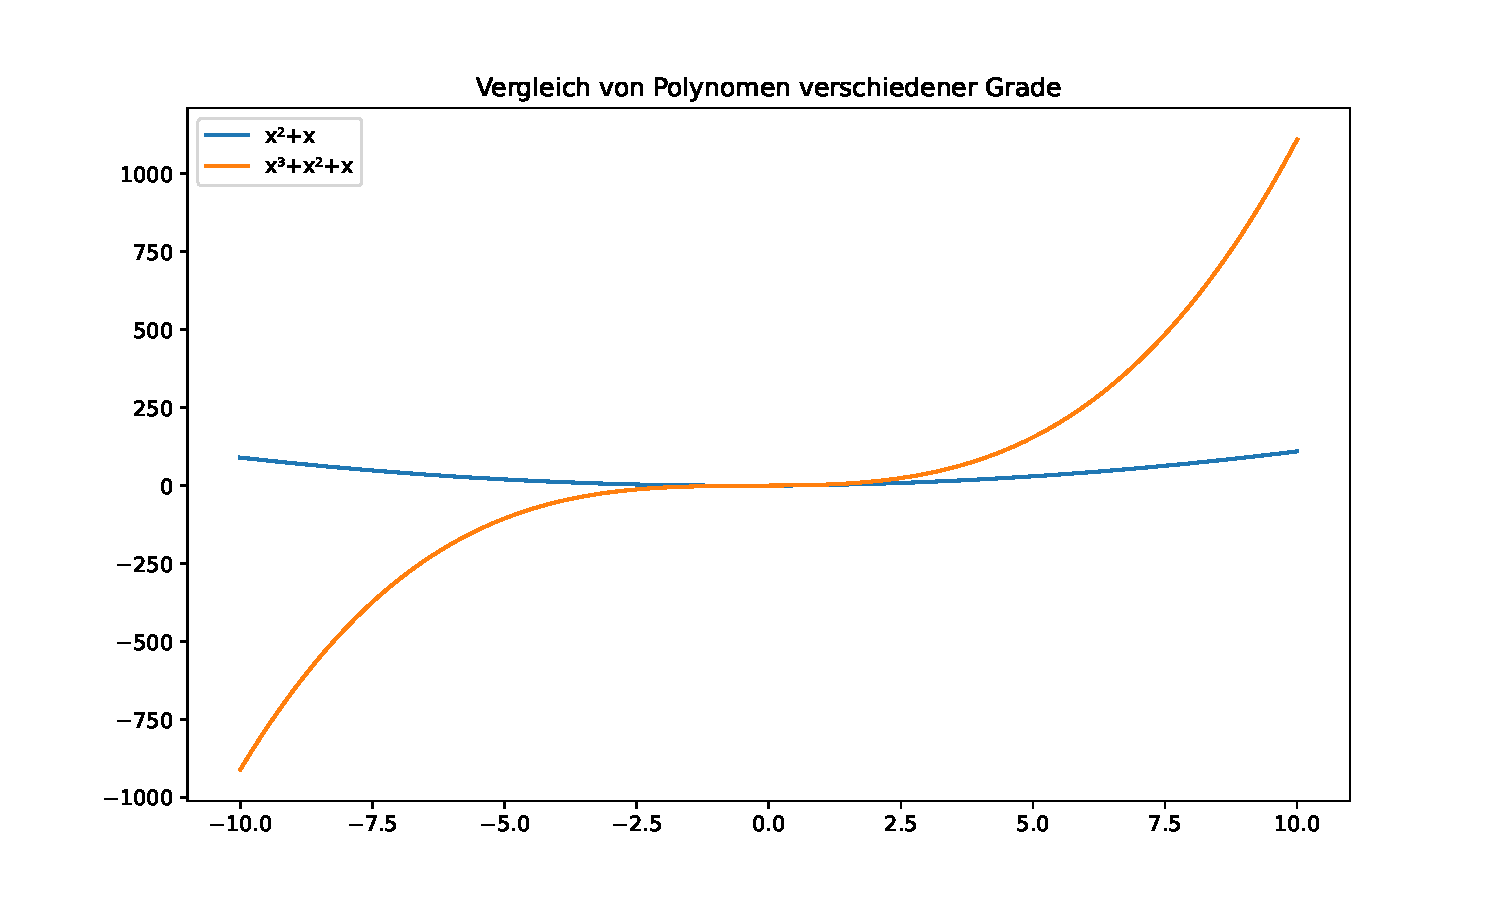
\includegraphics[width=0.7\textwidth]{Graphics/ComparissonDifferentPolDegrees.pdf}
  \caption{Vergleich von Polynomen verschiedener Grade}
  \label{fig:PolynomeVerschiedeneGrade}
\end{figure}

\subsection{Stückweise lineare Approximation}
Die stückweise lineare Approximation stellt einen Spezialfall der stückweisen polynomiellen Approximation dar, bei dem ausschließlich Polynome ersten Grades (also lineare Funktionen) zur Approximation der Segmente verwendet werden.
Durch die Beschränkung auf Grad 1 ergibt sich eine einfachere Funktionsform sowie geringerer Rechenaufwand, jedoch unter Umständen auch eine schlechtere Approximation komplexer Verläufe im Vergleich zu höhergradigen polynomiellen Approximationen.

\subsection{Diskrete Fourier-Transformation}
Die \ac{DFT} ist ein mathematisches Verfahren zur Zerlegung einer endlichen, diskreten Zeitreihe in ihre Frequenzteile. Das heißt für eine gegebene Zeitreihe $[(t_0,x_0),(t_1,x_1),\ldots,(t_{n-1},x_{n-1})]$ gibt \acs{DFT} eine neue Liste, mit den Frequenzen von 0 bis $n-1$, zurück. Für diese Transformation ist folgende Formel definiert:
\[y_k=\sum_{\ell=0}^{n-1}x_\ell\,e^{i\,\tfrac{2\pi k}{n}\,\ell},\]
wobei $[y_0,y_1,\ldots,y_{n-1}]$ die neue Liste ist und $i$ die imaginäre Einheit.

Was dieses Verfahren tut, lässt sich gut an einem Beispiel zeigen. In \autoref{fig:dftKomplettBeispiel} sieht man in Grün ein Signal, das aus drei sich überlagernden Frequenzen erstellt wurde. Die blauen Punkte sind zwölf Messpunkte einer Zeitreihe, die dieses Signal abgetastet hat, und die orangenen Kreuze sind die Beträge des Ergebnisses der \acs{DFT}. 
\begin{figure}[bth] 
  \centering
  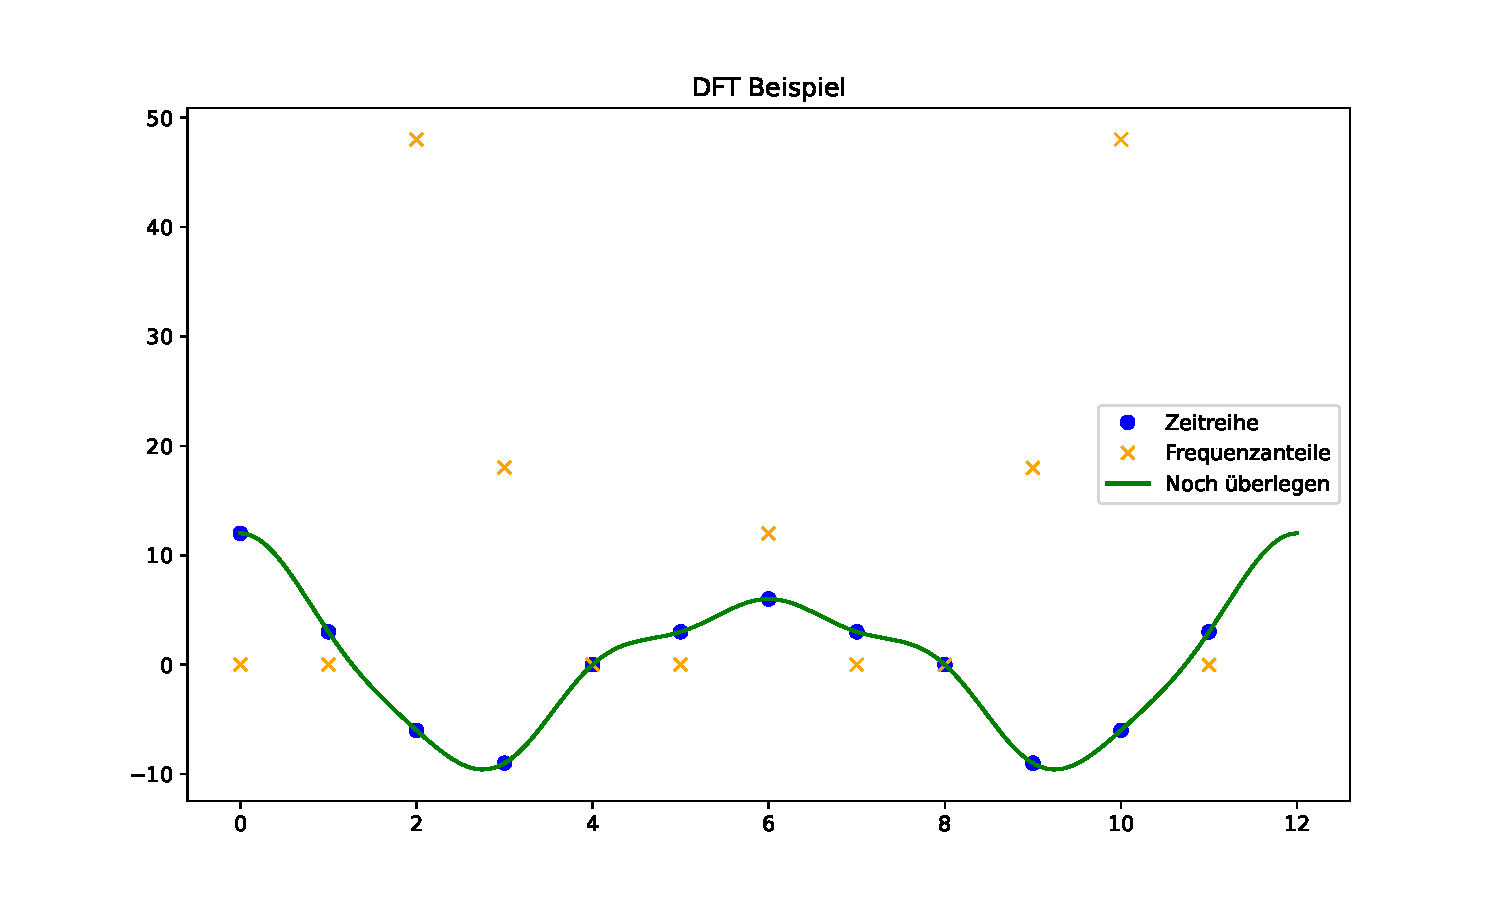
\includegraphics[width=0.7\textwidth]{Graphics/DFTExample1.pdf}
  \caption{Beispiel einer diskreten Fourier"=Transformation}
  \label{fig:dftKomplettBeispiel}
\end{figure}

In \autoref{fig:dftEinzelneFrequenzen} sieht man nun die drei ursprünglichen Frequenzen, die überlagert das Signal aus \autoref{fig:dftKomplettBeispiel} ergeben. Die blauen Punkte und orangenen Kreuze zeigen auch hier das abgetastete Signal beziehungsweise die Beträge des Ergebnisses der \acs{DFT}. Durch die Aufteilung in die drei einzelnen Bilder wird klar, was die \acs{DFT} eigentlich macht. Sie extrahiert aus dem ursprünglichen Signal diese drei Frequenzen und speichert mittels einer komplexen Zahl Informationen über die Amplitude und Phasenverschiebung der jeweiligen Frequenz. So sieht man in \autoref{subfig:dft2}, dass beide Amplituden bei 48 liegen. Da die \acs{DFT} diese Werte nicht normalisiert, müssen sie, nachdem sie addiert wurden, durch $n=12$ dividiert werden. Wir erhalten eine Amplitude von 8, was durch Betrachtung des grünen Graphens bestätigt werden kann. Selbiges gilt für \autoref{subfig:df3} und \autoref{subfig:dft4}, wo die addierten Amplituden 36 beziehungsweise 12 ergeben und die normierten 3 beziehungsweise 1.
\begin{figure}[bth]
  \subfloat[Erste Frequenz]{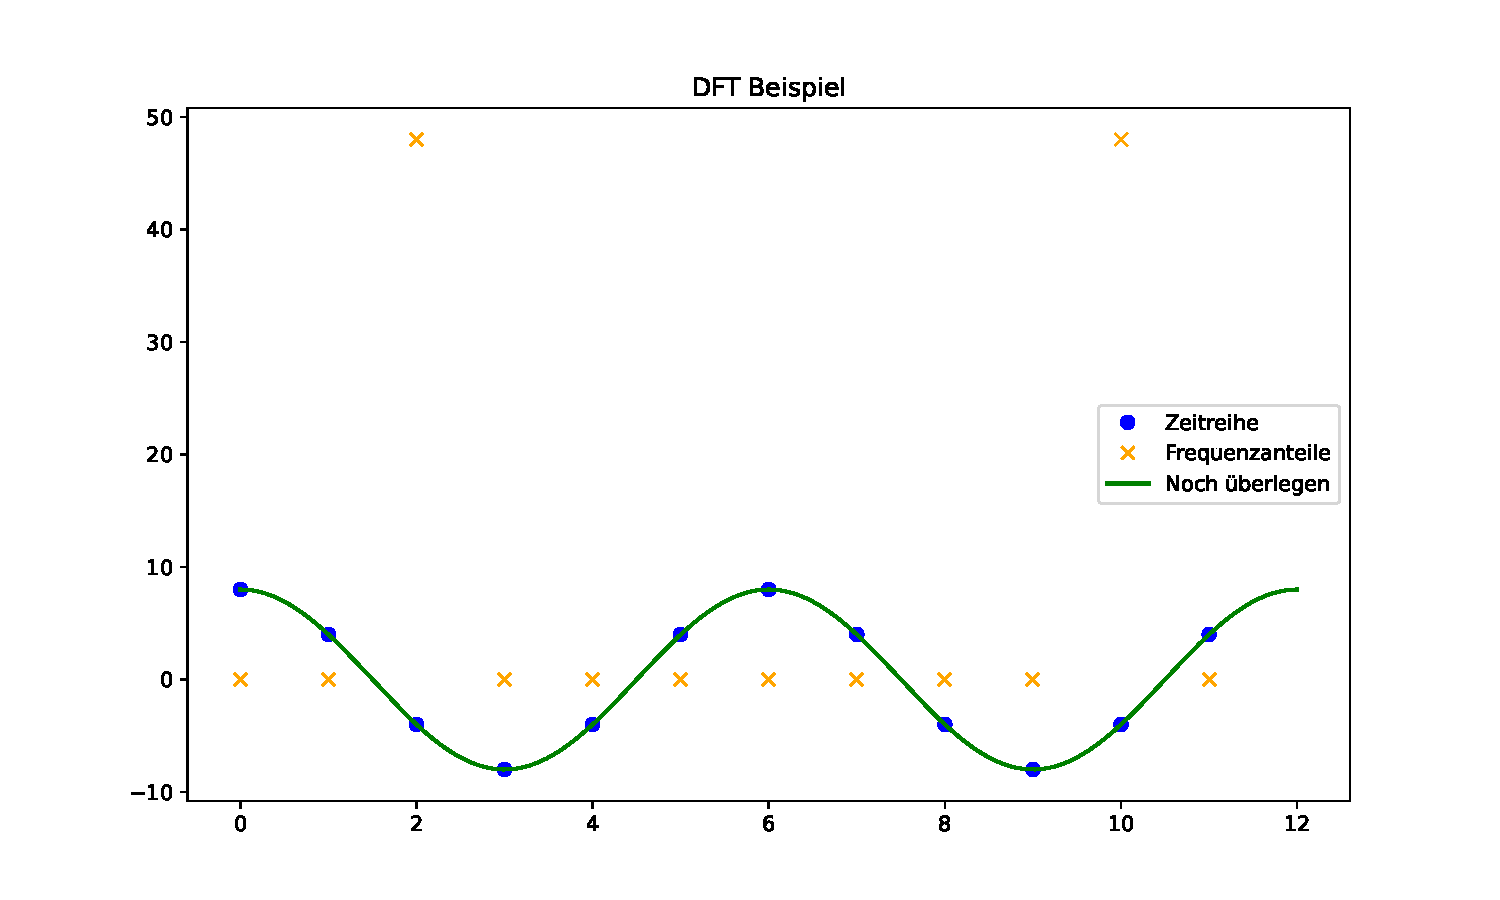
\includegraphics[width=0.49\textwidth]{Graphics/DFTExample4.pdf}\label{subfig:dft2}}\hfill
  \subfloat[Zweite Frequenz]{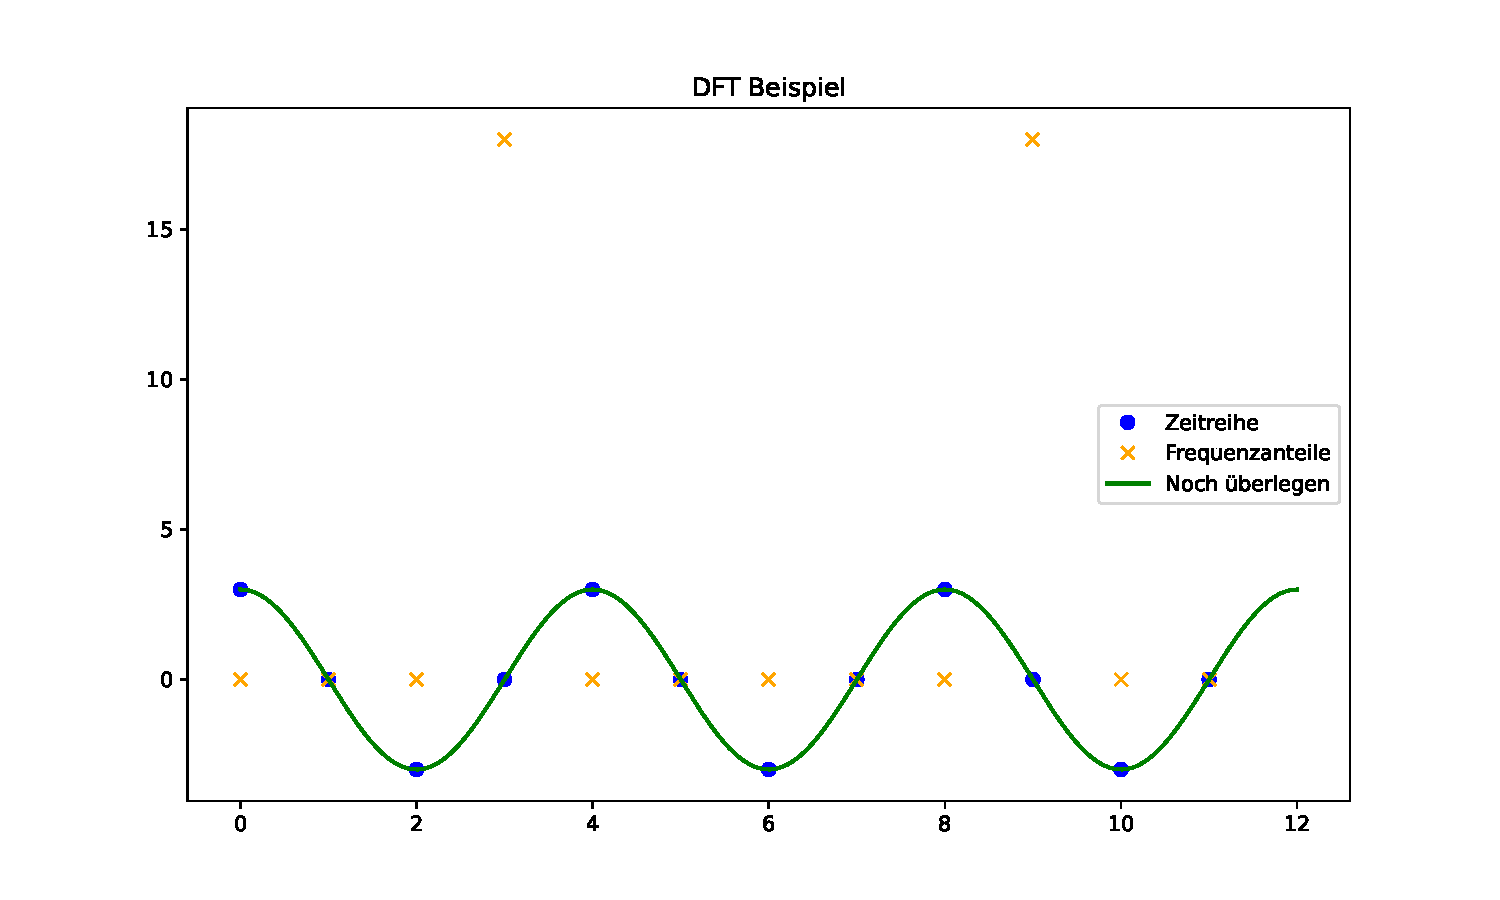
\includegraphics[width=0.49\textwidth]{Graphics/DFTExample3.pdf}\label{subfig:df3}}\hfill
  \centering\subfloat[Dritte Frequenz]{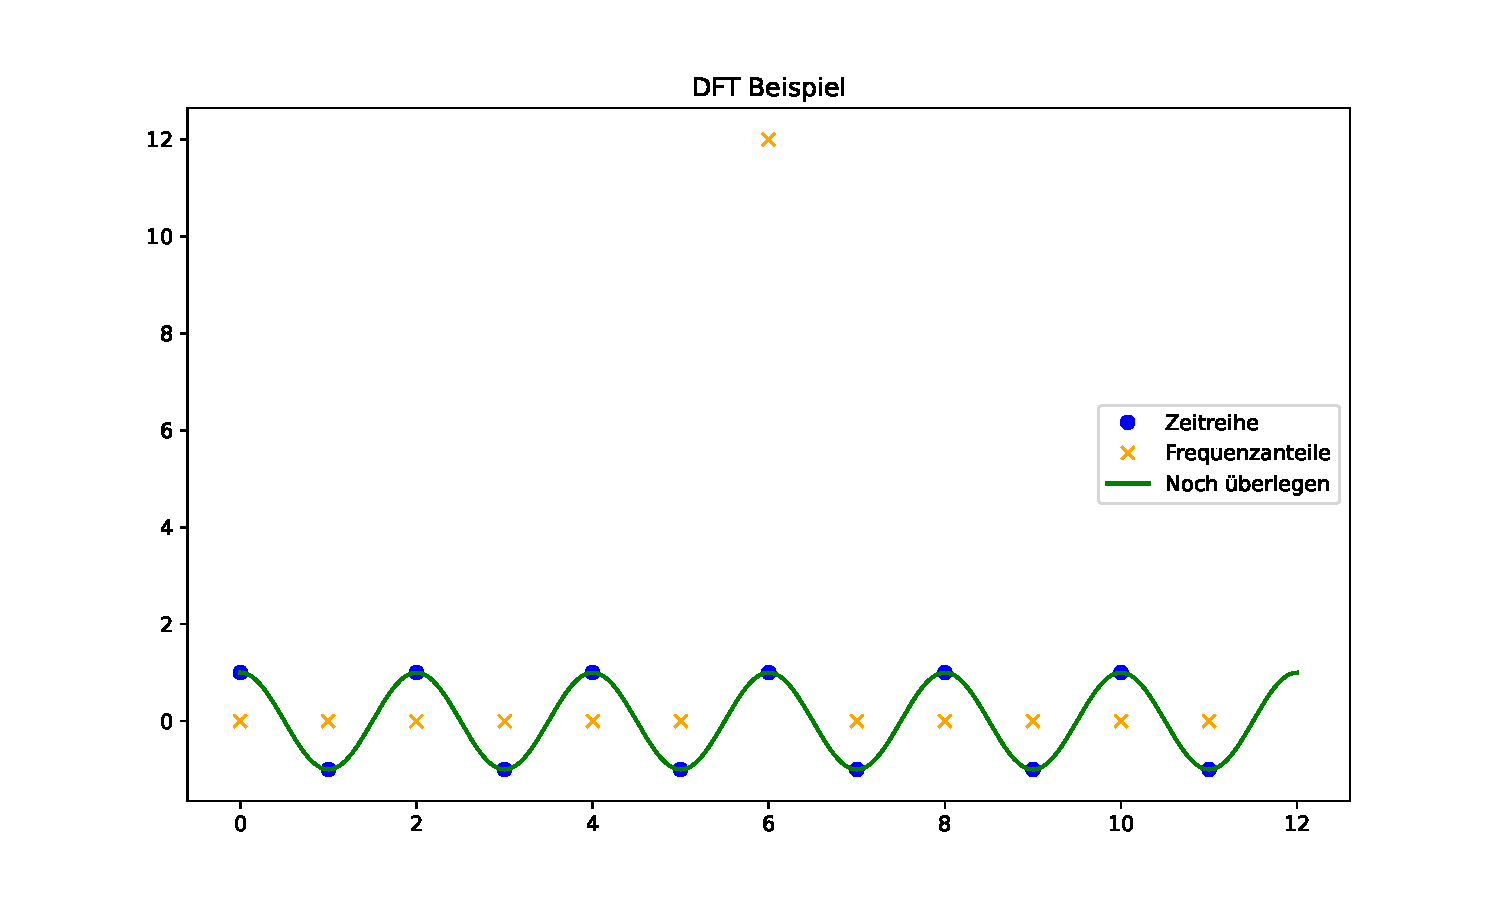
\includegraphics[width=0.49\textwidth]{Graphics/DFTExample2.pdf}\label{subfig:dft4}}
  \caption{Ursprüngliche Frequenzen der Überlagerung aus \autoref{fig:dftKomplettBeispiel}}
  \label{fig:dftEinzelneFrequenzen}
\end{figure}

Zum besseren Verständnis der am Anfang genannten Formel wird in diesem Abschnitt nun näher auf die Mathematik dahinter eingegangen. In der Formel handelt es sich wegen der imaginären Einheit $i$ um komplexe Zahlen. Diese bestehen aus einem Realteil $a$ und einem Imaginärteil $b$, also in der Form $a + ib$. Sie können allerdings auch als Punkt in einer zweidimensionalen Ebene interpretiert werden, dann liegt der Realteil typischerweise auf der x-Achse und der Imaginärteil auf der y-Achse. Außerdem gibt es die Exponentialform $a+ib=re^{i\varphi}$, wobei $r$ der Abstand vom Ursprung zum Punkt $(a,b)$ ist und $\varphi$ der Winkel, den diese Strecke mit der positiven x-Achse einschließt. $r$ wird auch Betrag genannt und wird folgendermaßen berechnet: $r=\sqrt{a^2+b^2}$. Setzt man nun $r=1$ und lässt $\varphi$ von 0 bis $2\pi$ laufen, erhält man einen Einheitskreis. Unterteilt man diesen Kreis jetzt in $n$ gleich große Abschnitte ein, so kann man mit $e^{i\frac{2\pi k}{n}}$ über $n$ diskrete Punkte iterieren, wobei $k$ eine natürliche Zahl von 0 bis $n-1$ ist. Auffallen dürfte an dieser Stelle, dass dieser Term dem aus der obigen Summenformel entspricht. Setzt man also nun, entsprechend unseres Beispiels in \autoref{fig:dftKomplettBeispiel}, $n=12$, so erhält man einen Einheitskreis, der mit dem in \autoref{fig:komplexerEinheitskreis} übereinstimmt. Diese 12 Punkte werden dann mittels des restlichen Terms der \acs{DFT}, mit den Datenpunkten gewichtet.
\begin{figure}[bth] 
  \centering
  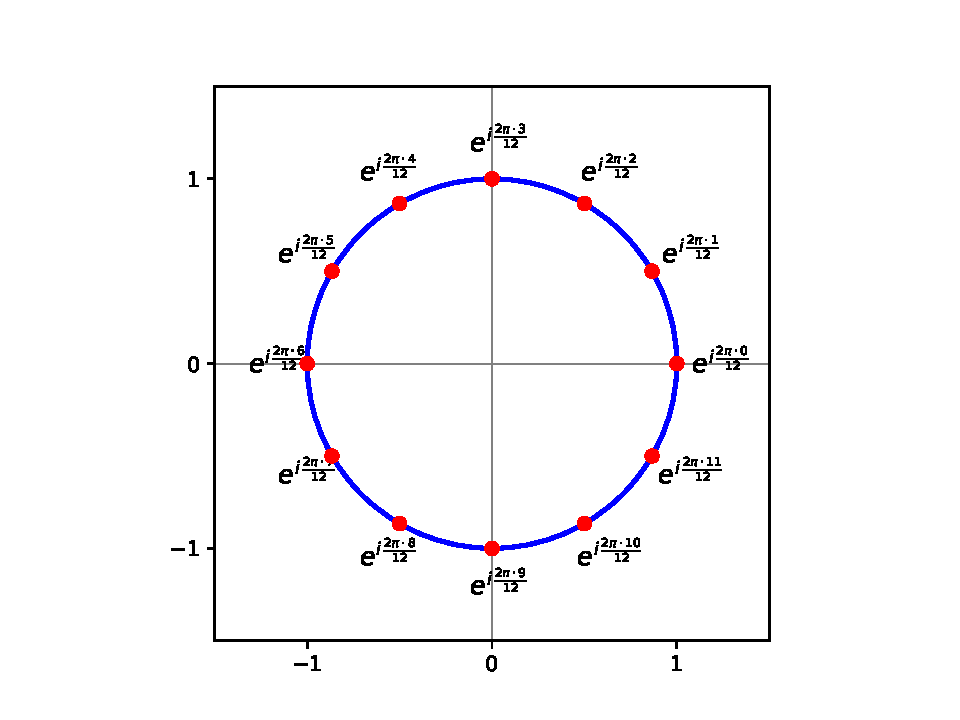
\includegraphics[width=0.7\textwidth]{Graphics/KomplexerEinheitskreis.pdf}
  \caption{Einheitskreis mit zwölf gleich großen Abschnitten}
  \label{fig:komplexerEinheitskreis}
\end{figure}

\subsection{Diskrete Wavelet"=Transformation}
\blindtext
\section{Verfahren zur Ausreißererkennung}
Verfahren zur Ausreißererkennung bewerten die übergebenen Daten mithilfe eines Ausreißer"=Scores, der ihre Wahrscheinlichkeit bewertet, ein Ausreißer zu sein. Die Verfahren in den ersten zwei Abschnitten können von diesem Score allerdings nicht direkt ableiten, ob ein Datenpunkt ein Ausreißer ist oder nicht, sondern sie geben einen festgelegten Prozentsatz zurück, der Datenpunkte, die am schlechtesten abschneiden. Im dritten und letzten Abschnitt wird dann ein Verfahren präsentiert, das selber einen Schwellwert festlegt, ab dem es einen Punkt als Ausreißer markiert, das kann auch dazu führen, dass keine Ausreißer gefunden werden, nicht wie bei den ersten beiden Verfahren.

\subsection{k"=Nearest"=Neighbors}
Das k"=Nearest"=Neighbors oder knn Verfahren zur Ausreißererkennung von Sridhar Ramaswamy et al. \cite{knn}, erkennt Ausreißer dadurch, dass sie eine größere Distanz zu anderen Punkten besitzen. Um die Distanz zu berechnen wird in der verwendeten Bibliothek PyOD \cite{pyod} die Minkowski"=Distanz \cite{minkowski} benutzt, die zwischen zwei Punkten $x = (x_0,x_1,\ldots,x_{n-1})$ und $y=(y_0,y_1,\ldots,y_{n-1})$ die Distanz $d(x,y)$ wie folgt berechnet:
\[d(x,y) = \left(\sum_{i=0}^{n-1}|x_i - y_i|^p\right)^{\frac{1}{p}}.\]
Der Parameter $p$ wird von PyOD standardmäßig auf 2 gesetzt, wodurch wir einen Spezialfall der Minkowski"=Distanz erhalten, und zwar die Euklidische"=Distanz, die auch beim Maß der Ähnlichkeit in \autoref{subsec:aehnlichkeit} benutzt wird. Was knn nun macht ist, dass es von allen Punkten, die Abstände zu allen anderen Punkten berechnet und für jeweiligen Punkt speichert. Daraufhin merkt es sich nur die $k$"=Stück die am nächsten sind und setzt den Ausreißer"=Score auf die Distanz des am weitesten entfernt, unter den $k$"=Stück. Punkte mit einem hohen Ausreißer"=Score, haben weniger Punkte, die dicht an ihnen dran sind und sind somit offensichtlich Ausreißer. PyOD setzt außerdem standardmäßig den Wert $k=5$. Upmanu Lall und Ashish Sharma \cite{kauswahl}, sowie Shichao Zhang et al. \cite{kauswahl2} nutzen ebenfalls diesen Wert, versuchen allerdings möglichst effizient ein optimales $k$ für einen gegebenen Datensatz zu finden. Da $k=5$ de facto ein etablierter Standardwert ist und genauere Analysen über die Auswirkung des Parameters umfangreich sind \cite{kauswahl2} und nicht zentral für diese Arbeit, da es nicht um die Optimierung des Algorithmus, sondern um die Auswirkungen der Kompression geht, wird er in der Implementierung nicht geändert.

\subsection{Isolation Forest}
Das Isolation Forest oder iForest Verfahren zur Ausreißererkennung von Fei Tony Liu et al. \cite{iForest}, erkennt Ausreißer dadurch, dass sie leichter von anderen zu isolieren sind. Isolieren bedeutet hierbei das Abgrenzen eines Punktes von Anderen. Ausreißer sind leichter abzugrenzen, da sie zwei Eigenschaften besitzen:
\begin{enumerate}
    \item "`Ausreißer sind eine Minderheit, die aus wenigen [Datenpunkten] besteht"',
    \item "`Sie besitzen Werte die sich stark von denen, von normalen [Datenpunkten] unterscheiden"'
\end{enumerate}
(vergleiche \cite[Ch. 1]{iForest}, aus dem Englischen übersetzt) \\
iForest isoliert Datenpunkte, indem es sie zufällig rekursiv partitioniert, so lange bis nur noch ein Datenpunkt in einer Partition liegt. Diese zufällige Partitionierung sorgt dafür, dass Ausreißer mit nur wenigen Partitionen isoliert werden, da es nur wenige Datenpunkte sind, die sich von den anderen stark unterscheiden. Um diese Idee visuell zu verdeutlichen, veranschaulicht die \autoref{fig:partitionierungen} eine Isolierung von einem normalen Datenpunkt $x_i$ und von einem Ausreißer $x_0$. Dabei sind die kleinen Kreise die verschiedenen Datenpunkte und die schwarzen Linien die Grenzen der Partitionen. In \autoref{subfig:partitionierung1} sieht man nun, dass zur Isolierung von $x_i$ viele zufällige Partitionen benötigt werden. In \autoref{subfig:partitionierung2} sieht man wiederum, dass relativ schnell, mit nur zwei zufälligen Partitionen, $x_0$ isoliert werden konnte.
\begin{figure}[bth]
  \subfloat[Isolierung von $x_i$]{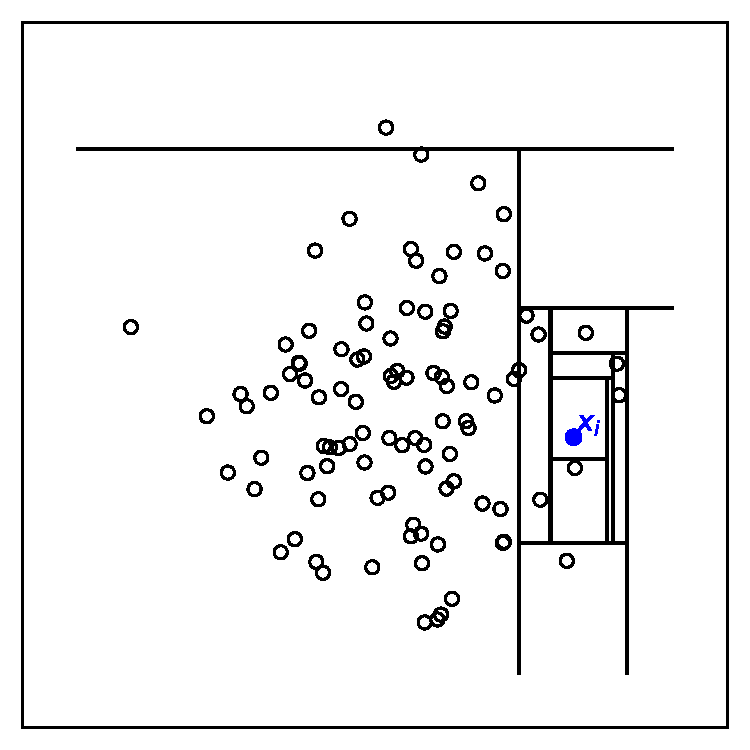
\includegraphics[width=0.49\textwidth]{Graphics/Partitionierung1.pdf}\label{subfig:partitionierung1}}\hfill
  \subfloat[Isolierung von $x_0$]{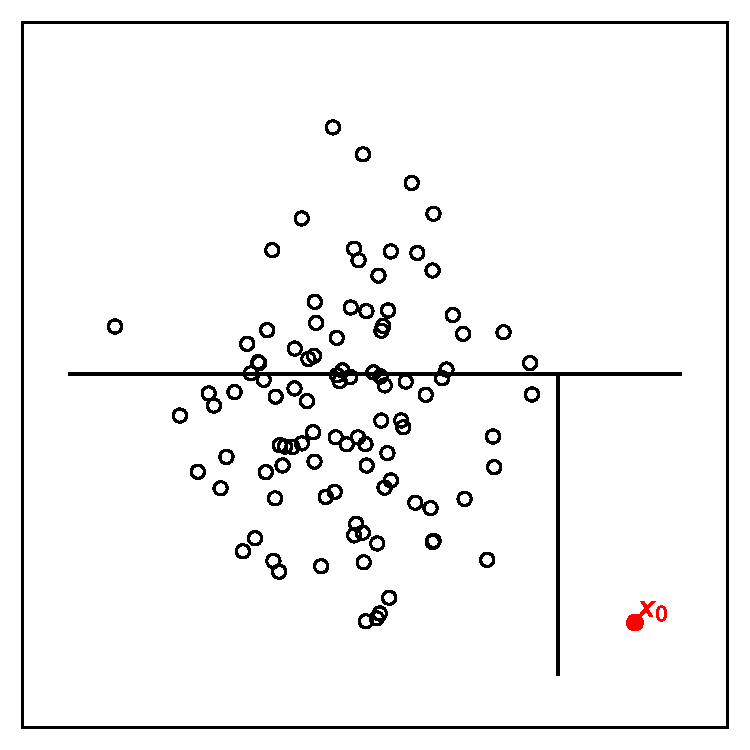
\includegraphics[width=0.49\textwidth]{Graphics/Partitionierung2.pdf}\label{subfig:partitionierung2}}\hfill
  \caption{Zufällige Partitionierung zur Isolierung zweier Punkte, angelehnt an \cite[Fig. 1]{iForest}}
  \label{fig:partitionierungen}
\end{figure}

Das rekursive Partitionieren lässt sich auch als Baum darstellen, wobei dann die Pfadlänge von der Wurzel zu einem Knoten genau der Anzahl der Partitionen entspricht. Daher kommt auch der Name iForest, da mehrere dieser Bäume zur Isolierung generiert werden, um, durch die zufällige Partitionierung, Partitionen mit verschiedenen Daten zu erhalten. Die durchschnittliche Pfadlänge der verschiedenen Datenpunkte ist dann die erwartete Pfadlänge. Die Baumstruktur baut sich wie folgt auf: Zuerst wird aus den Beobachtung in $ZR$ eine zufällige Teilmenge $X$ ausgesucht, meist nicht mehr als 256 Elemente, da dies zu genaueren Ergebnissen führt \cite[Ch. 4.1]{iForest}. Dann beginnt die Konstruktion des Baums, indem die Menge $X$ in die Wurzel des Baums geschrieben wird. Daraufhin wird ein zufälliges Feature ausgesucht und ein zufälliger Wert $p$, der zwischen dem Minimum und Maximum aus diesem Feature liegt. Die Menge $X$ wird dann entsprechend $p$ in zwei disjunkte Teilmengen aufgeteilt, wobei die kleineren Werte in den linken Kindknoten, und die größeren Werte in den rechten Kindknoten der Wurzel geschrieben werden. Die Schritte ab der Auswahl des zufälligen Features werden nun für die Kindknoten so lange fortgeführt, bis entweder:
\begin{itemize}
    \item "`der Baum eine maximale Höhe erreicht hat"',
    \item "`$|X|=1$"',
    \item beim zufällig ausgewählten Feature, "`alle Werte der Elemente in $X$  identisch sind"'.
\end{itemize}
(vergleiche \cite[Ch. 2]{iForest}, aus dem Englischen übersetzt) \\
Etwa 100 Bäume genügen \cite[Ch. 4.1]{iForest}, um keine signifikanten Unterschiede mehr in der durchschnittlichen Pfadlänge zwischen Wurzel und einem Knoten zu erhalten. Um dann einen zwischen Wurzel und einem Knoten zu erhalten. Um dann einen Ausreißer"=Score zu erhalten, wird folgende Formel angewandt:
\[ s(x,n)=2^{-\frac{E(h(x))}{c(n)}}, \]
wobei $|X|=n$, $c(n)=2H(n-1)-(2(n-1)/n)$, $H(i)=\ln(i) + 0,5772156649$ (Euler"=Mascheroni"=Konstante), $h(x)$ ist die Pfadlänge eines Knotens $x$ in einem Baum, also die Kantenanzahl von Wurzel bis zu diesem Knoten und $E(h(x))$ ist die durchschnittliche Kantenanzahl über alle Bäume. Diese Formel normalisiert die durchschnittliche Höhe und garantiert damit, dass wir immer $0 < s \le 1$ erhalten, für egal welches $n$ und $x$. Mit $s$ kann man nun drei Einschätzungen vornehmen:
\begin{itemize}
    \item "`ist das $s$ eines Knoten nah an 1, dann ist es definitiv ein Ausreißer"',
    \item "`ist das $s$ eines Knoten weit unter 0,5, dann kann man mit Sicherheit sagen, dass es ein normaler [Datenpunkt] ist"',
    \item "`geben alle [Datenpunkte] $s \approx 0,5$ zurück, dann gibt es keine auffälligen Ausreißer"'.
\end{itemize}
(vergleiche \cite[Ch. 2]{iForest}, aus dem Englischen übersetzt)

\subsection{Random Projections mit Median"=Absolute"=Deviation}
Dieses Verfahren orientiert sich stark an dem von Paula Navarro-Esteban und Juan Antonio Cuesta-Albertos \cite{randomProjection}. Es beruht auf der Idee, dass man multivariate Daten auf mehrere ein-dimensionale Werte projiziert und je Projektion eine univariate Ausreißererkennung anwendet. Projektion bedeutet hierbei, dass das Skalarprodukt zwischen zwei Vektoren berechnet wird. In unserem Kontext wird also das Skalarprodukt zwischen dem Vektor $x$ mit den Werten einer Zeitreihe und einem Vektor $y$ mit zufälligen, positiven Werten gebildet. Das Skalarprodukt entspricht der Summenformel $\sum_{i=1}^{n}x_iy_i$, wobei $n$ die Anzahl der Komponenten der Vektoren ist, beziehungsweise die Länge der Zeitreihe. Der Grund dieser Projektion ist, dass Zeitreihen die ähnliche Werte haben, auch ähnliche Projektionswerte besitzen, Zeitreihen, die sich komplett anders verhalten, haben wiederum stark abweichende Projektionswerte. 

Was das Verfahren also nun macht ist, dass es einen Vektor mit zufälligen, positiven Werten erstellt und diesen mit allen Zeitreihen verknüpft, um eine Liste an Projektionswerten zu erhalten. Auf diese Liste wird dann, wie in \cite[Ch. 3.3]{randomProjection}, das univariate Ausreißererkennungs"=Verfahren Median"=Absolute"=Deviation angewendet. Diese Erstellung eines zufälligen Vektors, mit anschließender Projektion und Ausreißererkennung, wird jetzt 50 Mal wiederholt, da dies ein Wert ist, der für keinen hohen Rechenaufwand sorgt und gleichzeitig ausreichend hoch ist, um die Zufallseffekte einzelner Projektionen zu glätten und stabile, reproduzierbare Ergebnisse bei der Ausreißererkennung zu gewährleisten \cite[Ch. 4.1]{randomProjection}. In einer separaten Liste wird gespeichert wie oft eine Zeitreihe als Ausreißer erkannt wurde. Diese Liste wird wieder mithilfe von Median"=Absolute"=Deviation auf Ausreißer untersucht, damit Zeitreihen die z.~B. nur ein einziges Mal als Ausreißer erkannt wurden, und damit wahrscheinlich kein echter Ausreißer sind, nicht als Ausreißer zurückgegeben wird.

Median"=Absolute"=Deviation ist ein simples Verfahren um auf univariaten Daten Ausreißer zu erkennen \cite[Ch. 3.3]{mad}. Für die univariaten Daten $X=x_0,x_1,\ldots, x_{n-1}$ wird zuerst der Median berechnet: \[\text{Median}(X)=\left\{ \begin{array}{ll}
    x_{\frac{n-1}{2}} & \text{falls } n \text{ ungerade} \\
    0,5 (x_{\frac{n}{2}-1} + x_{\frac{n}{2}}) & \text{falls } n \text{ gerade} \\
\end{array} \right.,\] dann wird der Median der absoluten Abweichungen um den Median der Daten (MAD) berechnet, heißt für jedes Element $x_i$ in $X$, wird die Differenz $|x_i - \text{Median}(X)|$ berechnet und der Median der Menge dieser Differenzen ist der MAD"=Wert. Nun wird ein Schwellwert $d$ festgelegt, der multipliziert mit dem MAD"=Wert den Bereich um den Median der Daten festlegt, in dem keine Ausreißer liegen. Heißt ein Wert $x_i$, der $\text{Median(X)} - d \cdot \text{MAD} < x_i < \text{Median}(X) + d \cdot \text{MAD}$ erfüllt, ist ein normaler Wert, wenn nicht, ist es ein Ausreißer. Boris Iglewicz und David C. Hoaglin \cite[Ch. 3.3]{mad} empfehlen auf Grundlage ihrer eigenen Studie einen Schwellwert von $d=3,5$, während Christoph Leys et al. \cite[p. 766]{mad2} Schwellwerte von 3, 2,5 und 2 vorschlägt, in einem darauffolgenden Abschnitt aber auch feststellt, dass in seinem Beispiel etwa 3,5 ein optimaler Wert ist. 